\documentclass[a4paper,10pt,parskip]{scrartcl}
\usepackage[utf8]{inputenc}
\usepackage[ngerman]{babel}
\usepackage[T1]{fontenc}
\usepackage{lmodern}
\usepackage{amsmath}
\usepackage{amsfonts}
\usepackage{amssymb}
\usepackage{amsthm}
\usepackage{siunitx}
\usepackage{epsfig}
\usepackage{url}
\usepackage{tikz}
\usepackage[lined,algoruled,linesnumbered]{algorithm2e}
%% \usepackage{algpseudocode}
%% \usepackage{algorithm}
\usepackage{graphicx}
\usepackage{placeins}

% an seitenbreite angepasste tabellen
\usepackage{booktabs}
\usepackage{tabularx} % page-width
\usepackage{adjustbox}

% coole inline-todos :)
\usepackage[colorinlistoftodos,prependcaption]{todonotes}

\renewcommand{\arraystretch}{1.5}

\usetikzlibrary{shapes.geometric, positioning, calc, shapes, fit, backgrounds}

\title{Projektausarbeitung \\\vspace{.5cm} \large gt Scaffolder: Eine Scaffolding-Software}

\author{Dorle Osterode, Lukas Götz \& Stefan Dang}
\date{}

\begin{document}
\maketitle{}
\thispagestyle{empty}
\begin{abstract}
  \todo{wollen wir ein abstract haben?}
\end{abstract}

\newpage{}
\thispagestyle{empty}
\tableofcontents{}
\newpage{}
\setcounter{page}{1}
\section{Einleitung}
\todo{Das Scaffolding Problem}

Das Ziel einer DNA-Sequenzierung ist die Bestimmung der Basen-Abfolge der vorliegenden DNA. Moderne Sequenzierungstechniken, auch Sequenzierung der zweiten Generation genannt, liefern typischerweise Reads als Paare. Dabei wird jeweils vom Ende eines DNA-Fragments sequenziert. Abhängig vom verwendeten Sequenzierungsprotokoll überbrücken gepaarte Reads Lücken (Inserts) variabler Größe.

Zur Rekonstruktion der Zielsequenz aus den Reads unabhängig von einer Referenzsequenz kann eine \textit{de novo} Assemblierung durchgeführt werden. Typischerweise wird hierbei in zwei Schritten vorgegangen: Zunächst werden die einzelnen Reads zu durchgängigen Sequenzen (Contigs) assembliert. Dabei kann das Zielgenom oftmals noch nicht vollständig rekonstruiert werden. Aufgrund teilweise unzureichender Abdeckung durch die Sequenzierung sowie repititive Teilsequenzen entstehen Lücken (Gaps), welche zu unabhängigen Contigs zu führen, deren relative Anordnung und Orientierung zueinander nicht bestimmt werden kann.

Durch \textit{Paired-End}- oder \textit{Mate-Pair}-Sequenzierung gewonnene Reads können hierbei mehrere Contigs überbrücken und so eine Beziehung zwischen diesen herstellen. Im zweiten Schritt einer \textit{de novo} Assemblierung können diese Distanzinformationen dazu verwendet werden, um die Contigs in Scaffolds anzuordnen. Dies erhöht die Durchgängigkeit der assemblierten Sequenz.
Das Scaffolding Problem kann als graphentheoretisches Problem formuliert werden. Dabei repräsentieren die Knoten des Graphen die einzelnen Contigs. Zwischen zwei Knoten existiert eine Kante, falls ein Read-Paar existiert, welches die beiden Contigs verbindet. Kanten enthalten dabei Informationen über die Distanz und die Orientierung der Read-Paare zueinander. Die Ermittlung eines Scaffolds, nämlich des optimalen Pfades (Pfad mit maximalem Kantengewicht) jeder Zusammenhangskomponente des Scaffolding Graphen, ist NP-schwer~\cite{Huson:2002kf}. Daher verwenden aktuelle Strategien eine Heuristik, um einen ausreichend guten Pfad zu bestimmen.

(\todo{Alternativer Vorschlag})

Nach der Assemblierung von Sequenzen ist das Zielgenom oftmals noch
nicht vollständig rekonstruiert. Die rekonstruierten Sequenzabschnitte
(Contigs) sind dabei unabhängig voneinander und die relative Anordnung
sowie die Orientierung sind unbekannt. Diese Lücken (Gaps) in der
Zielsequenz entstehen oft durch ungleichmäßige Abdeckung durch die
Sequenzierung sowie repetitive Teilsequenzen. Durch repetitive
Teilsequenzen können die Contigs nicht in eine eindeutige Reihenfolge
gebracht werden.

Durch das Scaffolding nach der Assemblierung sollen die Contigs
relativ zueinander angeordnet werden, sodass zusätzlich auch die
Orientierung stimmt. Um dieses Verfahren anwenden zu können müssen
Distanzinformationen zwischen den Contigs vorhanden sein. Diese
Informationen stammen normalerweise aus \textit{paired-end}- oder
\textit{mate-pair}-Sequenzierung.

Beim Scaffolding wird ein Graph zur Repräsentation der Beziehungen
zwischen den Contigs verwendet. Dieser Graph enthält für jeden Contig
einen Knoten und es gibt Kanten zwischen zwei Knoten, wenn es ein
Read-Paar gibt, dass die durch die Knoten repräsentierten Contigs
verbindet. Die Kanten enthält dabei Informationen über die Distanz und
die Orientierung.

Nach Huson (2002) \cite{Huson:2002kf} ist das Scaffolding Problem
NP-vollständig. Dabei ist das Scaffolding die Ermittlung des optimalen
Pfades (Pfad mit maximalem Kantengewicht) jeder
Zusammenhangskomponente des Scaffolding-Graphen. Um diese Komplexität
zu umgehen werden Heuristiken zur Bestimmung eines guten Pfades für
jede Zusammenhangskomponente verwendet.

\section{Ziel des Projektes und Arbeitsvorgehen}
\subsection{Ziel des Projektes}
Die Implementierung und Evaluierung einer Scaffolding-Software stellte
das allgemeine Projektziel dar. Dabei sollten die in der
GenomeTools-Bibliothek \cite{Gremme:2013} vorhandenen Konzepte und
Infrastruktur verwendet und eine Kompatibilität mit den Ausgaben des
Assemblers Readjoiner \cite{Gonnella:2012gn} gewährleistet werden. Der
Scaffolder aus dem SGA-Softwarepaket \cite{Simpson:2012ef} sollte als
Vorlage dienen, da diese Software im Rahmen einer Untersuchung
verschiedener Scaffolding-Programme Ergebnisse mit besonders hoher
Qualität lieferte \cite{Hunt:2014dh}. Andererseits enthält
SGA-Scaffold zahlreiche Abhängigkeiten zu nicht-Standardsoftware, die
durch die Reimplementierung minimiert werden sollten. Dazu gehört zum
Beispiel, dass zur Ermittelung der Distanzinformationen eine Zuordnung
der Reads zu den Contigs auf Basis des String-Graphen erfolgt anstelle
eines Read-Mappings durch BWA \cite{Li:2009}. Des Weiteren existiert
keine hinreichende Dokumentation der Methodik von SGA-Scaffold, so
dass dessen Aufklärung einen zentralen Teil des Projektes umfasste.

\subsection{Arbeitsvorgehen}
Zuerst wurden die verwendeten Datenformate und die Algorithmen
aufgeklärt. Da diese nicht hinreichend dokumentiert waren, mussten
diese Informationen aus dem Source-Code \cite{source} extrahiert werden.

Die so erhaltene Vorlage wurde leicht modifiziert, um sowohl Laufzeit
als auch Speicherplatz einzusparen. Unklarheiten in der Methodik wurden
dabei weitestgehend erst übernommen, um die Ergebnisse reproduzieren
zu können.

Diese Algorithmen wurden in der Programmiersprache C
implementiert. Dabei wurde gt Scaffolder zuerst so designet, dass es
die gleichen Eingabedateien erforderte wie SGA-Scaffold und die
gleichen Ausgaben produzierte, damit die Ergebnisse verglichen werden
konnten.

Um die Implementation zu testen wurden verschiedene Testdaten
ausgesucht. (\todo{hier mehr dazu schreiben!!!})

Anhand der Testdaten wurde gt Scaffolder evaluiert.

\section{Methoden}
\label{sec: Methoden}
\subsection{Übersicht der Schritte}

\begin{figure}
    \begin{tikzpicture}[every node/.style={font=\footnotesize}]
    \node[] (input1) {Contigs};
    \node[left of=input1, xshift=-1cm] (eingabe) {\textbf{Eingabe:}};
    \node[below of=eingabe, yshift=-5cm] (ausgabe) {\textbf{Ausgabe:}};
    \node[right of=input1, align=center, xshift=2cm] (input2) {Distanz-\\informationen};
    \node[right of=input2, xshift=2cm] (input3) {A-Statistik};

    \node[below of=input1, yshift=-.5cm, anchor=west] (titel) {gt Scaffolder};
    \node[rectangle, draw, anchor=west, below of=titel, xshift=1cm, rounded corners, fill=black!10, yshift=.25cm] (konstruktion) {Konstruktion des Graphen};
    \node[rectangle, draw, anchor=west, below of=konstruktion, xshift=.95cm, rounded corners, fill=black!10, yshift=.25cm] (selektion) {Selektion relevanter Knoten und Kanten};
    \node[rectangle, draw, anchor=west, below of=selektion, xshift=.80cm, rounded corners, fill=black!10, yshift=.25cm] (ermittlung) {Ermittlung aller Zusammenhangskomponenten (ZK)};
    \node[rectangle, draw, anchor=west, below of=ermittlung, xshift=-.65cm, rounded corners, fill=black!10, yshift=.25cm] (pfade) {Bestimmung des besten Pfades für jede ZK};

    \begin{pgfonlayer}{background}
    \node[draw, fit={(titel) (konstruktion) (selektion) (ermittlung) (pfade)}, rounded corners, fill=black!20] (back) {};
    \end{pgfonlayer}

    \node[below of=back, yshift=-2cm, xshift=-1.5cm] (output1) {Scaffolds};
    \node[right of=output1, align=center, xshift=2cm, yshift=-.25cm] (output2) {(rekonstruierte\\Sequenzen)};
    \node[above of=output1] (dummy) {};

    \path[->, thick]
    (input1) edge (back)
    (input2) edge (back)
    (input3) edge (back)
    (back) edge (output1)
    (back) edge (output2);
  \end{tikzpicture}
    \caption{\label{abb: gtscaffolder}Schematische Darstellung des Programmablaufs von gt Scaffolder.}
\end{figure}

In Abbildung \ref{abb: gtscaffolder} ist der Programmablauf von gt
Scaffolder schematisch dargestellt. Als Eingabe werden drei Dateien
benötigt. Diese Dateien enthalten die Informationen zu den Contigs und
den Distanzen, die gebraucht werden um den Scaffold-Graph konstruieren
zu können. Mit dieser Eingabe wird zuerst der Graph
konstruiert. Anschließend die relevanten Knoten und Kanten selektiert,
indem die übrigen Knoten und Kanten markiert werden. Nach der
Ermittlung aller Zusammenhangskomponenten des Scaffold-Graph, wird für
jede Zusammenhangskomponente ein Pfad berechnet, der als Scaffold
ausgegeben wird.

Die einzelnen Schritte werden im Folgenden näher
beschrieben.

\subsection{Eingabe}
Als Eingabe werden die Contigs im FASTA-Format, die
Distanzinformationen aus der \textit{paired-end}-
bzw. \textit{mate-pair}-Sequenzierung und die Astatistik der einzelnen
Contigs benötigt. gt Scaffolder benötigt dabei die
Distanzinformationen bezogen auf die Contigs, d.h. die Read-Paare
müssen zurück auf die Contigs gemappt und daraus die Distanz- sowie
Orientierungsinformation für die Contigs berechnet worden sein. Die
Astatistik ist ein statistisches Maß dafür, wie repetitiv eine Sequenz
ist \cite{Myers:2005iq}.

\subsection{Graphkonstruktion}
Aus den Contigs und den Distanzinformationen wird der
Scaffolding-Graph konstruiert. Dabei wird für jeden Contig, der eine
Mindestlänge von 200 bp überschreitet und eine Astatistik größer 19
hat, ein Knoten in den Graph eingefügt. Die Distanzinformationen
werden genutzt um die Knoten miteinander über Kanten zu
verbinden. Dabei werden zwischen jedem Knotenpaar, zwischen dessen
repräsentierten Contigs eine Distanzinformation vorhanden ist, zwei
Kanten eingefügt, die jeweils Orientierung und Distanz angeben.

\subsection{Selektion relevanter Knoten und Kanten}
In dem konstruierten Graph werden relevante Knoten und Kanten
selektiert. Dazu werden nicht relevante Knoten und Kanten markiert und
im späteren Vorgehen nur unmarkierte Knoten und Kanten betrachtet. Es
werden folgende Kriterien überprüft:
\begin{itemize}
\item Polymorphe Knoten: Zwei Knoten werden gelten als polymorph, wenn
  diese sich bezüglich eines gemeinsamen Vorgängerknotens nicht
  eindeutig anordnen lassen. Zusätzlich muss die Kopiezahl beider
  Knoten gering genug sein. Der Knoten mit der geringeren Kopiezahl
  wird als polymorph markiert und nicht weiter betrachtet.
\item Inkonsistente Kanten: Zwei Kanten $e_1$ und $e_2$ gelten als
  inkonsistent, wenn sich die Endknoten $e_1.end$ und $e_2.end$ bei
  einer Anordnung bezüglich des gemeinsamen Startknotens $e_1.start =
  e_2.start$ mit mindestens 400 bp überlappen. Gehen von einem Knoten
  zwei inkonsistente Kanten aus, so werden alle ausgehenden Kanten als
  inkonsistent markiert.
\end{itemize}
Der Pseudocode zur Markierung polymorpher Knoten und inkonsistener
Kanten ist in Algorithmus \ref{alg: Selektion} dargestellt.

Zusätzlich werden noch gerichtete Zyklen aufgelöst. Dazu werden alle
Zusammenhangskomponenten des Graphen berechnet. Für jede dieser
Zusammenhangskomponente wird mit einer Tiefensuche nach Rückkanten
gesucht. Dabei wird diese Tiefensuche von jedem terminalen Knoten, ein
Knoten der nur ausgehende \textit{sense} oder \textit{antisense}
Kanten hat, aus gestartet. Wird eine Rückkante gefunden, so werden die
Kante und die durch die Kante verbundenen Knoten markiert.

Da sich durch die Entfernung einer Kante die Struktur des Graphen
verändert und immer nur ein Zyklus für jeden terminalen Knoten
aufgelöst wird, muss diese Prozedur so lange wiederholt werden bis
keine Zyklen mehr gefunden werden.

Der Pseudocode für diesen Filterungsschritt ist in Algorithmus
\ref{alg: Zyklen} abgebildet.

\subsection{Ermittlung des besten Pfades/ Scaffolding}

Nach der Reinigung des Graphen wird das eigentliche Scaffolding
durchgeführt. Dazu werden alle Zusammenhangskomponenten des Graphen
bestimmt, um für jede Zusammenhangskomponente die beste Anordnung der
repräsentierten Contigs zu berechnen. Für jede Zusammenhangskomponente
werden die kürzesten Pfade bezüglich der Kantengewichte zwischen
terminalen Knoten mit einer Breitensuche berechnet. Der kürzeste Pfad
mit der meisten Sequenzabdeckung wird als Scaffold für die
Zusammenhangskomponente gewählt.

Contigs, deren repräsentierende Knoten keine oder nur markierte Kanten
haben, werden ebenfalls als Scaffolds gewählt.

Der Pseudocode für die Berechnung des Scaffolds ist in Algorithmus
\ref{alg: Scaffold} dargestellt.

\subsection{Ausgabe}
Die ermittelten Scaffolds werden in dem gleichen Format ausgegeben,
wie bei SGA. In diesem Format (\textit{.scaf}) steht in jeder Zeile
ein Scaffold. Die einzelnen Contigs mit ihren Informationen sind dabei
mit Tabs getrennt. Ein Beispieleintrag ist in Abbildung \ref{abb:
  scaf} dargestellt. Der erste Eintrag in einer Zeile ist die Id des
Startcontigs. Für die darauffolgenden Contigs werden folgende
Informationen mit Kommata getrennt angegeben: Id des Contigs, Distanz
zu dem vorherigen Contig, Standardabweichung der Distanz, Orientierung
zu dem vorherigen Contig (0: gleicher Strang, 1: entgegengesetzter
Strang), (\todo{Information über die Lage des Reads aus dem Readpaar,
0: gleicher Strang, 1: entgegengesetzter Strang} )

\begin{figure}
\begin{verbatim}
contig-100070  contig-34044,-99,2.500000,0,1,  contig-29023,-23,3.700000,0,0,
\end{verbatim}
\caption{\label{abb: scaf}Beispielzeile aus der Ausgabe von gt
  Scaffolder für den \textit{C. elegans} Testdatensatz.}
\end{figure}

Zusätzlich wurde ein Modul geschrieben um die Sequenzen der
berechneten Scaffolds rekonstruieren zu können. Bei SGA ist dies
ebenfalls ein seperater Schritt. Um die Sequenzqualität zu verbessern
wird dabei versucht Überlappungen durch Sequenzalignments aufzulösen
und Lücken zwischen den Contigs durch Pfade im String-Graph zu
schließen. Die Rekonstruktion der Sequenzen ist in Abschnitt \ref{sec:
  Rekonstruktion} näher beschrieben.

% LG: "Implementation" wuerde ich in die Methoden verschieben?
\section{Implementation}
\label{sec: Implementation}
\subsection{Erstellen der Distanzinformationen}
In gt Scaffolder können die Distanzinformationen explizit durch eine
Datei im ABySS-Distance-Format (*.de) angegeben werden. Eine solche
Datei wird durch das Programm DistEst von ABySS nach dem Assemblierungs-
und Read-Mapping Schritt in der SGA-Pipeline erstellt und dient als
Eingabe der Distanzinformationen für SGA-Scaffold. In der Evaluierung wurde diese Option für Vergleiche zwischen gt Scaffolder und SGA-Scaffold
verwendet.

Des Weiteren besteht die Möglichkeit, die Distanzinformationen aus
einer Datei im BAM-Format (*.bam) mit Hilfe eines Moduls zu
extrahieren. Dafür wurde das Programm DistEst von ABySS in C nach
implementiert. Aus Zeitgründen ist es nicht gelungen ein Modul zu
entwickeln zur Erzeugung der BAM-Datei auf Basis des String-Graphen. Stattdessen muss ein Read-Mapping separat nach der Assemblierung
durchgeführt werden.

\subsection{Rekonstruktion der Sequenz}
\label{sec: Rekonstruktion}
Zur Rekonstruktion der Sequenzen der berechneten Scaffolds werden drei
Schritte für alle aufeinander folgende Contigs durchlaufen. Zuerst
wird versucht die Lücke (Gap) zwischen den Contigs anhand eines Pfades
in dem String-Graph zu schließen. Für diesen Schritt wird der
String-Graph aller Contigs verwendet. Konnte kein eindeutiger Pfad nach
bestimmten Kriterien gefunden werden, so wird überprüft, ob die
Contigs sich überlappen. Ist die Distanz zwischen den Contigs negativ,
so werden die sich überlappenden Enden aligniert. Wenn kein Alignment
gefunden wurde, wird die Lücke mit Wiederholungen des Buchstaben 'N'
aufgefüllt.

Die gesamte Sequenz eines Scaffolds wird anhand dieser drei Schritte
folgendermaßen rekonstruiert. Die komplette Sequenz des ersten Contigs
wird übernommen. Danach wird für den jeweils nächsten Contig versucht
einen eindeutigen Pfad der richtigen Länge zwischen dem vorherigen und
diesem Contig im String-Graph zu finden. Anschließend wird versucht
bei negativer Distanz zwischen den Contigs ein Alignment zu finden,
sonst wird die Lücke zwischen den Contigs mit einer Reihe von
'N'-Symbolen aufgefüllt. Bei diesem Vorgang wird die relative
Orientierung der Contigs zueinander und zum ersten Contig beachtet und
die Sequenzen dementsprechend umgedreht \todo{anderes wort!}
bzw. komplementiert. Im Folgenden werden die einzelnen
Schritte näher beschrieben.

\subsubsection{Traversierung des Stringgraphen}
Nach der Assemblierung wird in SGA ein String-Graph im \textit{.asqg}
Format (siehe \cite{asqg}) ausgegeben. Dieser String-Graph wird mit
einem Python-Skript in das \textit{.spm} Format umgeschrieben.

Wie in Abbildung \ref{abb: spm} dargestellt, ist das \textit{.spm}
Format ein Zeilenbasiertes Format. In jeder Zeile ist ein
Suffix-Präfix-Match eingetragen. Die erste Zahl repräsentiert den
einen Contig oder Read, das folgende Zeichen gibt den Strang an ('+'
steht für den sense-Strang und '-' für den antisense-Strang), die
zweite Zahl repräsentiert den zweiten Contig oder Read, das folgende
Zeichen gibt den Strang an und die letzte Zahl entspricht der Länge
der Überlappung. Die Zahlen für die Contigs oder Reads entsprechen
dabei der Sequenznummer des Contigs oder Reads in einer GtEncseq.

\begin{figure}
  \centering
\begin{verbatim}
24129 + 0 + 148
1 + 85225 - 123
39261 - 1 + 137
2 + 27698 + 149
\end{verbatim}
\caption{\label{abb: spm}Beispielzeilen aus der \textit{.spm}-Datei des
  String-Graphen für den \textit{C. elegans} Testdatensatz.}
\end{figure}

Mit dieser Repräsentation des String-Graphen, der aus der
Assemblierung resultiert, wird der String-Graph wieder aufgebaut, in
dem die \textit{.spm}-Datei mit Infrastruktur, die in den Readjoiner
zugrundeliegenden Bibliotheken vorhanden ist, eingelesen wird.

Der String-Graph wird anschließend für jedes Paar an
aufeinanderfolgende Contigs $c_1$, $c_2$ in jedem Scaffold mit einer
Breitensuche traversiert. Es wird versucht einen eindeutigen Pfad von
Contig $c_1$ zu Contig $c_2$ in dem String-Graph zu finden. Dabei wird
überprüft, ob die Distanz zwischen den Contigs, die im Scaffolding
ermittelte Distanz nicht überschreitet. Um eine Traversierung des
gesamten String-Graphen zu verhindern, wird die Suche nach \num{10000}
besuchten Knoten abgebrochen. Ein gefundener Pfad wird dabei
verworfen, da die Eindeutigkeit nicht garantiert werden kann. Wird
mehr als ein Pfad zwischen den Contigs gefunden, wird die Suche
ebenfalls ohne Ergebnis abgebrochen.

Wurde ein eindeutiger Pfad gefunden, so wird der Pfad von $c_1$ zu
$c_2$ gespeichert und anschließend die Sequenz des Pfades anhand einer
GtEncseq der Contigs rekonstruiert. Diese rekonstruierte Sequenz wird
schließlich zurückgegeben.

\subsubsection{Berechnung von Alignments}
Ist die Distanz zwischen zwei im Scaffold benachbarten Contigs $c_1$
und $c_2$ negativ, so überlappen sich die Contigs theoretisch. Um
diese Überlappung in der Sequenz aufzulösen, wird ein Alignment
zwischen den Contigs $c_1$ und $c_2$ berechnet. Dabei wird das beste
Alignment genutzt, um die Sequenz zu rekonstruieren.

Es wird eine schon vorhandene Implementation des
Smith-Waterman-Algorithmus für lokale Alignments \cite{smith}
verwendet. Der Sequenzbereich der Contigs, in dem Alignments gesucht
werden, wird dabei durch die im Scaffolding ermittelte Distanz und das
dreifache der Standardabweichung festgelegt. Der Sequenzbereich wird
natürlich auch durch die Länge der beiden Contigs mit
festgelegt. Maximal werden allerdings höchsten je 500 Basen zur
Berechnung des Alignments verwendet, um zu hohen Rechenaufwand zu
vermeiden. Diese Maximallänge wurde von SGA übernommen.

Nur Suffix-Präfix-Überlappungen von Contig $c_1$ mit Contig $c_2$
werden betrachtet, wenn Contig $c_1$ im Scaffold direkt vor Contig
$c_2$ kommt. Die maximale erlaubte Fehlerrate (ergibt sich aus der
maximal erlaubten Edit-Distanz des Alignments und der Länge der
längsten eingehenden Sequenz) ist $max\_error = 0.05$ nach dem
standardmäßig bei SGA verwendeten Wert. Ebenso wurde die Mindestlänge
eines Alignments auf 20 Basen festgelegt.

Von allen gefundenen den Kriterien entsprechenden Alignments, wird das
Alignment mit der kleinsten Edit-Distanz gewählt. Ist $l$ die Länge
des besten Alignments und $seq_{c_2}$ die Sequenz des Contigs $c_2$,
so wird die Sequenz ab der Position $l$ ($seq_{c_2}[l:|seq_{c_2}|]$)
zurückgegeben. Falls kein hinreichendes Alignment gefunden werden
konnte, muss der nächste Schritt durchgeführt werden.

\subsubsection{Lücke schließen}
Konnte die Lücke zwischen zwei Contigs $c_1$ und $c_2$ nicht durch
eine Graph-Traversierung oder ein Alignment geschloßen werden, so wird
in diesem Schritt die Sequenz mit 'N's aufgefüllt. Dabei gibt es eine
Fallunterscheidung anhand der Distanz.

Ist die ermittelte Distanz zwischen $c_1$ und $c_2$ positiv, so wird
die Sequenz von $c_2$ nicht verändert. Vor die Sequenz werden der
Distanz entsprechend viele 'N'-Symbole geschrieben, jedoch mindestens
25.

Ist die ermittelte Distanz zwischen $c_1$ und $c_2$ negativ, so wird
der Präfix von $c_2$ der Länge 25 durch die gleiche Anzahl an
'N'-Symbolen ersetzt.

\section{gt Scaffolder als Tool in den GenomeTools}
Die in den Abschnitten \ref{sec: Methoden} und \ref{sec:
  Implementation} vorgestellte Funktionalität wurde in Form eines
Tools in die GenomeTools eingebunden. In Abbildung \ref{abb: help} ist
die Hilfe-Ausgabe des Tools gt Scaffolder dargestellt. Dabei sind alle
einstellbaren Parameter mit ihren standardmäßigen Belegungen zu sehen.

\begin{figure}
\begin{verbatim}
$ gt scaffolder -help
Usage: gt scaffolder [option ...] [file]
Constructs scaffolds of the contigs.

-min_contig_len    minimal contig length for used contigs
                   default: 200
-rep_cp_cutoff     minimal copy number for not repetitiv contigs
                   default: 0.30
-rep_astat_cutoff  minimal A-statistics for not repetitiv contigs
                   default: 20.00
-p_cutoff          probability cutoff for polymorphic vertices
                   default: 0.01
-cp_cutoff         copy num cutoff for polymorphic vertices
                   default: 1.50
-overlap_cutoff    overlap cutoff for inconsistent edges
                   default: 400
-contigs           contigs in FASTA format
                   default: undefined
-dist              distanceinformation in ABySS .de format
                   default: undefined
-astat             A-statistics file in SGAs .astat format
                   default: undefined
-spm               basename of spm-representation of used string-graph
                   default: undefined
-bam_min_qual      minimal quality in bam file
                   default: 10
-bam_min_nof_pairs minimal number of pairs
                   default: 10
-bam_min_dist      minimal distance of contigs
                   default: -99
-bam_max_dist      maximal distance of contigs
                   default: 9223372036854775807
-bam_min_align     minimal alignment length
                   default: 100
-bam               bam file containing alignments of paired reads to the contigs
                   default: undefined
-help              display help and exit
-version           display version information and exit

Report bugs to <gt-users@genometools.org>.
\end{verbatim}
\caption{\label{abb: help}Hilfeausgabe des Tools gt Scaffolder.}
\end{figure}

Die Optionen -contig und entweder -dist oder -bam sind
verpflichtend. Wird mit der Option -dist eine Distanzdatei in dem
erforderlichen Format übergeben, so wird diese eingelesen und die
Informationen verwendet. Wird mit der Option -bam eine BAM-Datei mit
Alignments der Reads zu den Contigs übergeben, so werden aus der
BAM-Datei die Distanzinformationen berechnet und in dem erforderlichen
Format gespeichert. Diese neuerzeugte Datei wird anschließend
eingelesen und die enthaltenen Informationen verwendet. Durch die
Möglichkeit eine BAM-Datei anzugeben wird die Abhängigkeit zu einem
Mapping-Programm (z.B. BWA \cite{BWA}) und einem Teil des
Assemblers ABySS \cite{abyss} durchbrochen. Aus dem in den
GenomeTools vorhandenen String-Graph Assembler Readjoiner können die
Informationen, welche Reads mit den Contigs aligniert werden können ,
direkt ausgegeben und somit als Eingabe für gt Scaffolder verwendet
werden.

Mit der Option -astat kann zusätzlich ein Datei mit Informationen über
die Astatistik und die berechneten Kopiezahlen der Contigs übergeben
werden. Diese Option wird für die Kompabilität mit der Eingabe von SGA
Scaffold benötigt. Sollen Contigs aus einer Assemblierung mit
Readjoiner verwendet werden, so kann mit der Option -astat von
Readjoiner direkt die Information in der Fasta-Datei der Contigs mit
angegeben werden. Wird gt Scaffolder ohne eine extra Astatistik-Datei
aufgerufen, so wird angenommen, dass diese Information in der
Fasta-Datei der Contigs enthalten ist.

Als Ausgabe wird Standardmäßig die \textit{.scaf}-Datei
erzeugt. Die Rekonstruktion der Sequenzen ist in dem Tool noch nicht
möglich, da die Erweiterung der String-Graph-API zur
Sequenzkonstruktion mittels Traversierung noch nicht in die
GenomeTools übernommen wurde.

\section{Änderungen zu bzw.\,komische Dinge in SGA Scaffold}

SGA benutzt eine relativ konservative Strategie, um vermeintlich
fehlerhafte Knoten und Kanten aus dem Scaffolding-Graph zu
entfernen. D.h. korrekte Knoten und Kanten werden lieber als
fehlerhaft eingestuft und entfernt, als dass fehlerhafte Knoten oder
Kanten nicht erkannt werden und in dem Endergebnis enthalten sein
könnten. Einige nicht sofort ersichtlichen Strategien von SGA wurden
zuerst in gt Scaffolder übernommen, um eine Vergleichbarkeit der
Ergebnisse der beiden Programme zu erhalten. Die Güte der Strategie
?\todo{wurde/muss/sollte was denn jetzt?} evaluiert werden.

Es folgt eine ungeordnete Auflistung solcher Strategien, teilweise um
mögliche Erklärungen ergänzt.
\begin{itemize}
\item Bei der Entfernung inkonsistenter Kanten eines Knoten $k_0$
  werden alle Kanten von den Nachbarknoten, die in der gleichen
  Richtung verlaufen wie die Kante vom Nachbarknoten zu $k_0$,
  ebenfalls entfernt. \\
  Mögliche Erklärung: Potentiell enthalten auch
  diese Kanten Inkonsistenzen und sollten deshalb nicht weiter
  betrachtet werden.
\item Bei der Konstruktion des Graphen wird zwischen zwei Knoten
  jeweils nur eine Kante eingefügt. Wenn es mehr als eine Kante geben
  würde wird die Kante mit der größten Standardabweichung
  gewählt. \\
  Mögliche Erklärung: keine.
\item Bei der Klassifikation der Knoten als repetitiv oder eindeutig
  wird zusätzlich zu der Astatistik auch die berechnete Anzahl an
  Kopien für jeden repräsentierten Contig betrachtet. Ein Knoten wird
  dabei als repetitiv markiert und später entfernt, wenn der die
  berechnete Anzahl an Kopien für den repräsentierten Contig zu gering
  ist. \\
  Mögliche Erklärung: Die Contigs mit einer zu geringen
  Kopiezahl sind potentiell fehlerhaft und sollten nicht betrachtet
  werden. Die Markierung als repetitiv ist dabei semantisch falsch und
  dient nur der späteren Entfernung des zugehörigen Knoten.
\end{itemize}

\section{Ergebnisse}

Zum Evaluieren und Testen der Implementierten Software wurden
verschiedene Testdatensätze ausgewählt. Die verwendeten Referenzgenome
sind in Tabelle \ref{tab: Referenzgenome} dargestellt.

\begin{table}
  \centering
  \begin{tabular}{l | c | l}
    Genom & Größe & Datensatzid \\
    \hline
    \textit{S. cerevisiae} & ~~12 Mbp & Ensembl R64-1-1 \\
    \textit{H. sapiens}, Chr. 21 & ~~48 Mbp & Ensembl GRCh37 \\
    \textit{C. elegans} & 100 Mbp & Ensembl WBcel235 \\
    \textit{D. melanogaster} & 140 Mbp & Ensembl BDGP5
  \end{tabular}
  \caption{\label{tab: Referenzgenome} Verwendete Referenzgenome mit
    ihrer Größe und den Datensatzids.}
\end{table}

Es wurden diese Referenzgenome gewählt, da sie sehr unterschiedliche
Größen haben. Die Größen decken einen Bereich von ca. 10 Mbp bis 140
Mbp ab, so dass die Entwicklung des Laufzeitverhaltens und des
Speicherplatzbedarfs über die Länge des Genoms betrachtet werden kann.

Mit dem Sequenzierungssimulator ART \cite{Huang:2012kq} wurde für jedes
der Genome eine \textit{paired-end}-Sequenzierung mit einem Illumina
Sequenzierer simuliert. Dabei wurde die Read-Länge auf 150 bp, die
Fragmentlänge auf 400 bp $\pm$ 10 bp und die Coverage wurde auf 20X
festgelegt.

Die so simulierten \textit{paired-end}-Reads wurden mit der
SGA-Pipeline assembliert und das so erhaltene Ergebnis für das
Scaffolding verwendet.

Die Berechnungen wurden auf einer Workstation durchgeführt. Die
technischen Daten sind: Core-i7 @ 3.10GHz, 8GB RAM, Linux 64 bit.

\subsection{Vergleich der Pipelines}

In Abbildung \ref{abb: Pipeline} sind die Assemblierungs- und
Scaffolding-Pipelines von SGA und gt Scaffolder dargestellt.

\begin{figure}
  \centering
  \begin{minipage}{.45\textwidth}
      \begin{tikzpicture}[node distance=.6cm]
        \tikzstyle{prog}=[draw, rectangle, rounded corners, font=\tiny];
        \node[prog] (prep) {preprocess};
        \node[prog, below of=prep] (index) {index};
        \node[prog, below of=index] (correct) {correct};
        \node[prog, below of=correct] (index2) {index};
        \node[prog, below of=index2] (filter) {filter};
        \node[prog, below of=filter] (overlap) {overlap};
        \node[prog, below of=overlap] (assemble) {assemble};
        \node[prog, right of=prep, xshift=1.5cm, fill=red!40] (bindex) {index};
        \node[prog, below of=bindex, fill=red!40] (aln) {align};
        \node[prog, below of=aln, fill=red!40] (sampe) {sampe};
        \node[prog, below of=sampe, rectangle split, rectangle split parts=3, yshift=-.45cm, rectangle split part fill={blue!40, green!40, blue!40}] (bam2de) {\nodepart{one}fixmate\nodepart{two}samtools\nodepart{three}DistanceEst};
        \node[prog, below of=bam2de, yshift=-.45cm, fill=yellow!40] (pysam) {astat};
        \node[prog, below of=pysam] (scaff) {scaffold};
        \node[prog, below of=scaff] (scaf2fasta) {scaf2fasta};

        \path[->]
        (prep) edge (index)
        (index) edge (correct)
        (correct) edge (index2)
        (index2) edge (filter)
        (filter) edge (overlap)
        (overlap) edge (assemble)
        (assemble.east) edge[in=180, out=0] (bindex.west)
        (bindex) edge (aln)
        (aln) edge (sampe)
        (sampe) edge (bam2de)
        (bam2de) edge (pysam)
        (pysam) edge (scaff)
        (scaff) edge (scaf2fasta);
      \end{tikzpicture}
    \end{minipage}
    \begin{minipage}{2cm}
      \begin{tikzpicture}[node distance=.6cm]
        \tikzstyle{prog}=[draw, rectangle, rounded corners, font=\tiny];
        \node[prog] (prefilter) {prefilter};
        \node[prog, below of=prefilter] (overlap) {overlap};
        \node[prog, below of=overlap] (assembly) {assembly};
        \node[prog, right of=prefilter, xshift=1cm] (scaffold) {scaffold};

        \path[->]
        (prefilter) edge (overlap)
        (overlap) edge (assembly)
        (assembly.east) edge[in=180, out=0] (scaffold.west);
      \end{tikzpicture}
    \end{minipage}
    \caption{\label{abb: Pipeline}Vergleich der Assemblierungs- und
      Scaffolding-Pipelines von SGA (links) und gt Scaffolder
      (rechts). In farbig sind Abhängigkeiten zu anderen Programmen
      oder externen Bibliotheken dargestellt.}
\end{figure}

\subsection{Evaluation der Ergebnisse}

In Tabelle \ref{tab: Vergleich} sind die Ergebnisse der Evaluation
dargestellt. Jeweils zwei Zeilen enthalten die Angaben zu einem
Referenzdatensatz. Dabei sind immer zuerst die Ergebnisse von SGA
Scaffold aufgetragen und in der Zeile darunter die Ergebnisse von gt
Scaffolder als Faktor. Zu jedem Datensatz ist in der ersten Spalte die
Anzahl an Contigs dargestellt, um die Größe des jeweiligen
Scaffoldgraphen zu skizzieren.

\begin{table}
  \adjustbox{max height=\dimexpr\textheight-5.5cm\relax, max width=\textwidth}{
    \begin{tabular}{llccccc}
      \toprule
      Datensatz & Programm & Abdeckung (Mbp / \%) & \#Scaffolds & N50 (kb) & CPU (s) & RAM (MB) \\
      \midrule
      \textit{S. cerevisiae}
      & SGA Scaffold  & ~~11.08 / 92  &     ~~600   &  32.3     & 0.01      &  28.9 \\
      1694 contigs
      & gt Scaffolder & $1\times$     &  $1\times$  & $1\times$ & $1\times$ &  $0.43\times$ \\
      \midrule
      \textit{H. sapiens}, Chr. 21
      & SGA Scaffold  & ~~34.25 / 71  &      1368   &  54.2     & 0.04  &  27.8  \\
      4817 contigs
      & gt Scaffolder & $1\times$     &  $1\times$  & $1\times$ & $1\times$ & $0.6\times$       \\
      \midrule
      \textit{C. elegans}
      & SGA Scaffold  & ~~94.07 / 94  &      5659   &  36.9     & 0.11  &  34.9 \\
      11113 contigs
      & gt Scaffolder & $1\times$     &  $1\times$  & $1\times$ & $0.9\times$ & $0.90\times$      \\
      \midrule
      \textit{D. melanogaster}
      & SGA Scaffold  & 113.48 / 81   &      2281   &  126.3    & 0.11    & 29.2     \\
      3970 contigs
      & gt Scaffolder & $1\times$     &  $1\times$  & $1\times$ & $0.9\times$ & $0.62\times$     \\
      \bottomrule
  \end{tabular}}
  \caption{\label{tab: Vergleich}Vergleich der Ergebnisse, der
    Laufzeit und des Speicherplatzbedarfs von gt Scaffolder und
    SGA-Scaffold.}
\end{table}

Die verglichenen Aspekte sind: Die Abdeckung des (\todo{welche
Abdeckung wurde betrachtet?!}) in Mbp und Prozent, die Anzahl an
berechneten Scaffolds, der N50 Wert der berechneten Scaffolds in kb,
die benötigte CPU-Zeit in Sekunden und der maximal benötigte
Speicherplatzbedarf in MB.

Der Faktor $1\times$ in den Spalten Abdeckung, \# Scaffolds und N50
zeigt an, dass gt Scaffolder und SGA Scaffold bei allen
Testdatensätzen die gleichen Ergebnisse produziert haben.

Bei der Laufzeit ist gt Scaffolder ungefähr genauso schnell wie SGA Scaffold. Der Faktor
$0.1\times$ um den gt Scaffolder bei den Testdatensätzen von
\textit{C. elegans} und \textit{D. melanogaster} schneller ist, ist
bei dieser Größenordnung nicht signifikant.

gt Scaffolder benötigt maximal um einen Faktor $0.1\times$ bis
$0.57\times$ weniger Speicherplatz bei der Berechnung der Scaffolds,
als SGA Scaffold.

\subsection{Vergleich der Laufzeit und des Speicherplatzbedarfs}
\begin{figure}[t]
  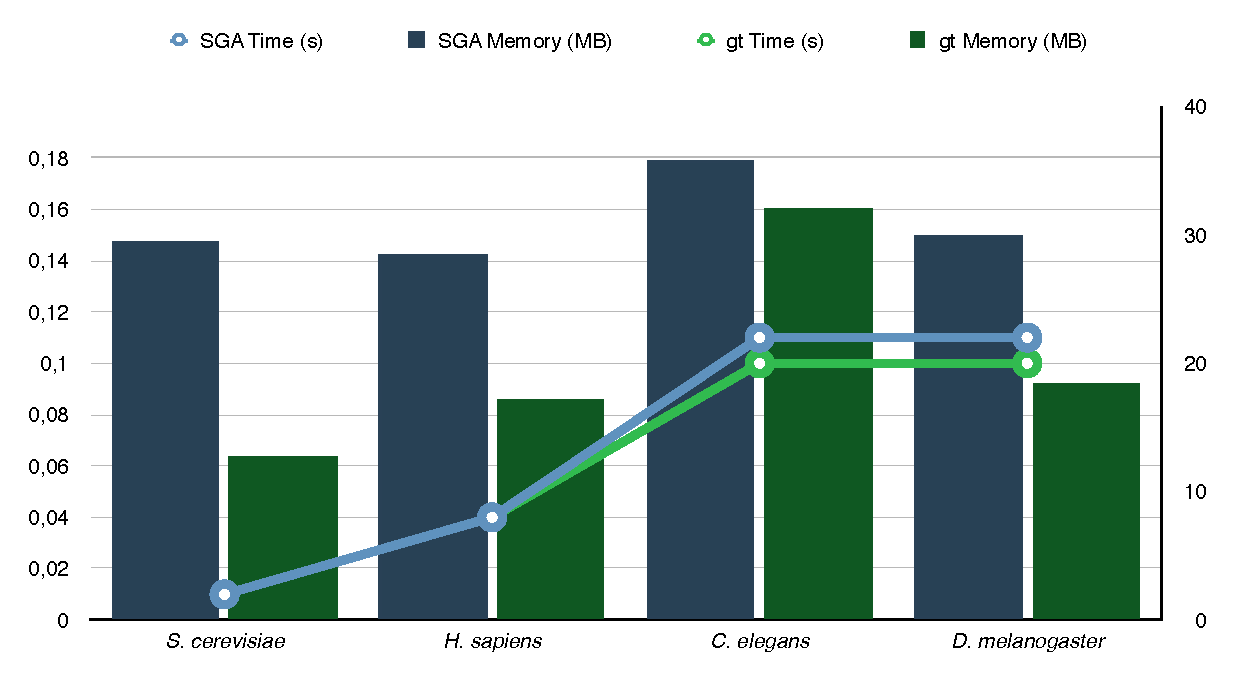
\includegraphics[width=\textwidth,height=0.8\textheight,keepaspectratio]{presentation/figures/sga_vs_gt.pdf}
  \caption{\label{abb: Zeit}Auftragung der Laufzeit und des
    Speicherplatzbedarfs von gt Scaffolder und SGA Scaffold für
    unterschiedliche Testdatensätze}
\end{figure}

In Abbildung \ref{abb: Zeit} sind die Laufzeiten und der
Speicherplatzbedarf der Programme gt Scaffolder und SGA Scaffold für
die verschiedenen Testdatensätze dargestellt. Die Testdatensätze sind
dabei der Größe nach von links nach rechts geordnet. Die Ergebnisse
von SGA Scaffold sind jeweils in rot dargestellt während die
Ergebnisse von gt Scaffolder grün eingefärbt sind.

Die Grafik verdeutlicht, dass gt Scaffolder sowohl bei der Laufzeit
als auch bei dem maximalen Speicherplatzbedarf entweder gleichauf mit
SGA Scaffold oder sogar besser ist.

Ebenfalls ist zu erkennen, dass die Laufzeit und der
Speicherplatzbedarf nicht mit der Größe der Referenzgenome
zusammenhängt. Allerdings hängen diese Punkte \todo{Punkte
  umformulieren?} auch nicht direkt von der Größe des Scaffoldgraphen
ab. In Tabelle \ref{tab: Vergleich} sind zu den Datensätzen die Anzahl
an Knoten in dem Scaffoldgraph dargestellt. So ist die Anzahl an
Knoten für den \textit{D. melanogaster} Datensatz mit $3970$ geringer
als für den \textit{H. sapiens} Chr. 21 Datensatz mit $4817$
Knoten. Trotzdem wird zur Berechnung der Scaffolds für den
\textit{D. melanogaster} Datensatz sowohl von SGA Scaffold als auch
von gt Scaffolder mehr Laufzeit und mehr Speicheplatz benötigt, wie
aus Tabelle \ref{tab: Vergleich} und Abbildung \ref{abb: Zeit}
ersichtlich wird. \todo{gehört dieser Abschnitt evtl in die Diskussion?}


\section{Diskussion und Ausblick}

\section*{Anhang}
\subsection*{Pseudocode}
(\todo{Algorithmen anpassen!!!})

\begin{algorithm}[H]
  \ForEach{Knoten $k_0$ im Graph $G$}{
    \ForEach{Kantenrichtung $dir$ in [ANTISENSE, SENSE]}{
      \ForEach{Kantenpaar $(e_0,e_1)$ in Richtung $dir$}{
        $k_1$ = $e_0.end$\;
        $k_2$ = $e_1.end$\;
        \If{AmbiguousOrdering($e_0,e_1,p\_cutoff$) \textbf{and}
           $k_1.copy\_num + k_2.copy\_num < cn\_cutoff$}
          {
            \If{$k_1.copy\_num < k_2.copy\_num$}{
              markiere $k_1$ und alle ein- und ausgehenden Kanten
              von $k_1$ als polymorph, wenn $k_1$ noch nicht markiert
              ist\;
            }
            \Else {
              markiere $k_2$ und alle ein- und ausgehenden Kanten
              von $k_2$ als polymorph, wenn $k_2$ noch nicht markiert
              ist\;
            }
           \tcp{bei polymorphen Knoten wird nur das erste
             polymorphe Kantenpaar markiert}
           \If{Knoten $k_0$ ist polymorph markiert}{
             break\;
           }
          }
        }
      \tcp{polymorphe Knoten müssen nicht mehr auf
        inkonsistente Kanten überprüft werden}
       \If{Knoten $k_0$ ist polymorph}
         {break\;}
       \ForEach{Kantenpaar $(e_0,e_1)$ in Richtung $dir$}{
         \If{$e_0$ ist nicht markiert und $e_1$ ist nicht markiert}
            {
              Berechne Überlappung von $e_0.end$ und $e_1.end$ und speichere
              längsten Überlappung.\;
            }
       }
       \If{längste Überlappung $>$ 400} {
	 Markiere alle ausgehenden Sense- bzw. Antisensekanten
         von $k_0$ und die eingehenden Kanten mit der Richtung der
         jeweiligen Zwillingskante als inkonsistent\;
      }
    }
  }
  \caption{\label{alg: Selektion}Filterfunktion zur Markierung von
    polymorphen Knoten und inkonsistenten Kanten. Die Funktion
    \textit{AmbigousOrdering} ist in Algorithmus \ref{alg: Order}
    dargestellt.}
\end{algorithm}
\todo{Zeile 13-15: das machen wir im code nicht!!! evtl wollen wir das aber machen!!!}

\begin{algorithm}[H]
  \KwData{Kante $e_0$ und Kante $e_1$, die auf eindeutige Ordnung geprüft werden
    sollen. Wahrscheinlichkeitsschwellenwert $p\_cutoff$}
  \KwResult{Ob die Kanten $e_0$ und $e_1$ nicht eindeutig geordnet werden können}
  $\mu = e_0.dist - e_1.dist$\;
  $\sigma^2 = e_0.std\_dev^2 + e_1.std\_dev^2$\;
  $t = \frac{-\mu}{\sigma\cdot\sqrt{2}}$\;
  $P_{e_0,e_1} = \frac{1}{2} \cdot \left( 1 + \frac{2}{\sqrt{\pi}} \int_{0}^{t} \exp{-x^2}\mathrm dx\right)$\;
  $P_{e_1,e_0} = 1 - P_{e_0,e_1}$\;
  \Return $\max\{P_{e_0,e_1}, P_{e_1,e_0}\} \leq p\_cutoff$
  \caption{\label{alg: Order}Funktion \textsc{AmbiguousOrdering}$(e_0, e_1, p\_cutoff)$}
\end{algorithm}


\begin{algorithm}[H]
  \KwData{Graph}
  \KwResult{Graph ohne Zyklen}
  \While{Zyklus gefunden wurde}{
  Suche alle Zusammenhangskomponenten $CC$\;
  \ForEach{Zusammenhangskomponente $C_0 \in CC$}{
    Suche alle terminalen Knoten $T$\;
    \ForEach{terminalen Knoten $t_0 \in T$}{
      Suche mit einer Tiefensuche von dem Knoten $t_0$ aus in der
      Richtung $t_0.edges[0].sense$ nach Rückkanten\;
      \If{Rückkante gefunden}{
        Markiere die Rückkante und die dadurch verbundenen Knoten
        als zyklisch\;
        }
      }
    }
  }
  \caption{\label{alg: Zyklen}Löse alle Zyklen für jede
    Zusammenhangskomponente auf}
\end{algorithm}

\begin{algorithm}[H]
  \SetAlgoLined
  \KwData{Graph $G$}
  \KwResult{Graph $G$ ohne Knoten, die nicht zum bestem Walk gehören}
  Markiere alle Kanten aus $G$ schwarz\;
  Berechnung der Menge $C$ aller Connected Components von $G$\;
  \ForEach{Connected Component $c_0$ aus der Menge $C$}{
    Berechne Menge der terminalen Knoten $T$ (mit ausschließlich SENSE
    oder ANTISENSE Kanten) für die Connected Component $c_0$\;
    \ForEach{Terminaler Knoten $t_0$ aus der Menge $T$}{
      Berechne die Menge $W$ aller Walks durch die Connected
      Component $c_0$ von $t_0$ aus\;
      \ForEach{Walk $w_0$ aus $W$}{
        \If{Contig-Gesamtlänge > bislang beste Contig-Gesamtlänge}{
          Setze aktuellen Walk $w_0$ als bestWalk\;
        }
      }
    }
  }
  Setze alle Kanten des bestWalk weiß\;
  Lösche alle schwarzen Kanten\;
  \caption{\label{alg: Scaffold}Berechnung der Scaffolds (Schritt 6)}
\end{algorithm}

\begin{algorithm}[H]
  \SetAlgoLined
  \KwData{terminaler Startknoten $t_0$}
  \KwResult{Alle von diesem Knoten möglichen Walks}
  Konstruktionsrichtung = Richtung der vom terminalen Knoten $t_0$ ausgehenden Kanten\;
  \ForEach{Kante $A$ vom Knoten $t_0$ ausgehend (in Konstruktionsrichtung)}{
    $k_0$ = $A.pend$\;
    Speichere Startkante $A$ und Distanz $A.dist$ in Map an Position
    $k_0$ (für spätere Traversierung)\;
    Schiebe Startkante $A$ und Distanz $A.dist$ in Queue\;
  }
  \While{BFS über Queue nicht beendet}{
    Poppe Kante $A$ und Distanz $A.dist$ aus der Queue\;
    $k_0$ = $A.pend$\;
    \ForEach{Kante $B$ in Konstruktionsrichtung von $k_0$ aus} {
      $k_1$ = $B.pend$\;
      \If{Distanz zu aktuell betrachtetem Knoten $k_1$ $<$
        bisher ermittelte Distanz zu $k_1$ {\bf OR} Knoten $k_1$
        noch unbetrachtet}{
        Speichere Kante $B$ und Distanz $B.dist$ in Map an Position $k_1$\;
        Schiebe Kante $B$ und Distanz $B.dist$ in Queue\;
      }
    }
    \If{$k_0$ hat keine Kanten in Konstruktionsrichtung}{
      Schiebe Knoten $k_0$ in terminalSet\;
    }
  }
  \ForEach{Knoten $k_0$ in terminalSet}{
    Erzeuge Walk mithilfe einer Traversierung über die Map
  }
  \caption{Berechnung der Walks (Schritt 6.1)}
\end{algorithm}

\bibliography{presentation/literatur}
\bibliographystyle{alpha}

\end{document}
